\documentclass[letterpaper,onecolumn,titlepage]{Ythesis}

\usepackage{graphicx}
\graphicspath{{sections/figs/}{.figs/}}

\usepackage[backend=bibtex, style=numeric-comp]{biblatex}
\bibliography{main}

\usepackage{subfiles}
\usepackage{url}
\usepackage{amsmath}



\title{Visualizing Conditional Relationships}
\author{Hannah Aizenman}
\committee{Dr. Michael Grossberg(Advisor), Dr. Robert Haralick, Dr. Huy Vo}
\submitted{}
\abstract{The context surrounding data is often as important as the
  measurements themselves. Income data provides a lens into demographic
  inequalities when separated by race and gender; temperature data indicates
  seasons when plotted by time. These are relatively simple relationships, but
 many datasets are embedded with rather complex conditional relationships. This
 survey gives an overview of techniques showing conditional dependencies
 amongst distributions and densities. 
}
\begin{document}
\makefrontmatter

\section{Introduction}
\label{sec:introduction}
\begin{figure}
  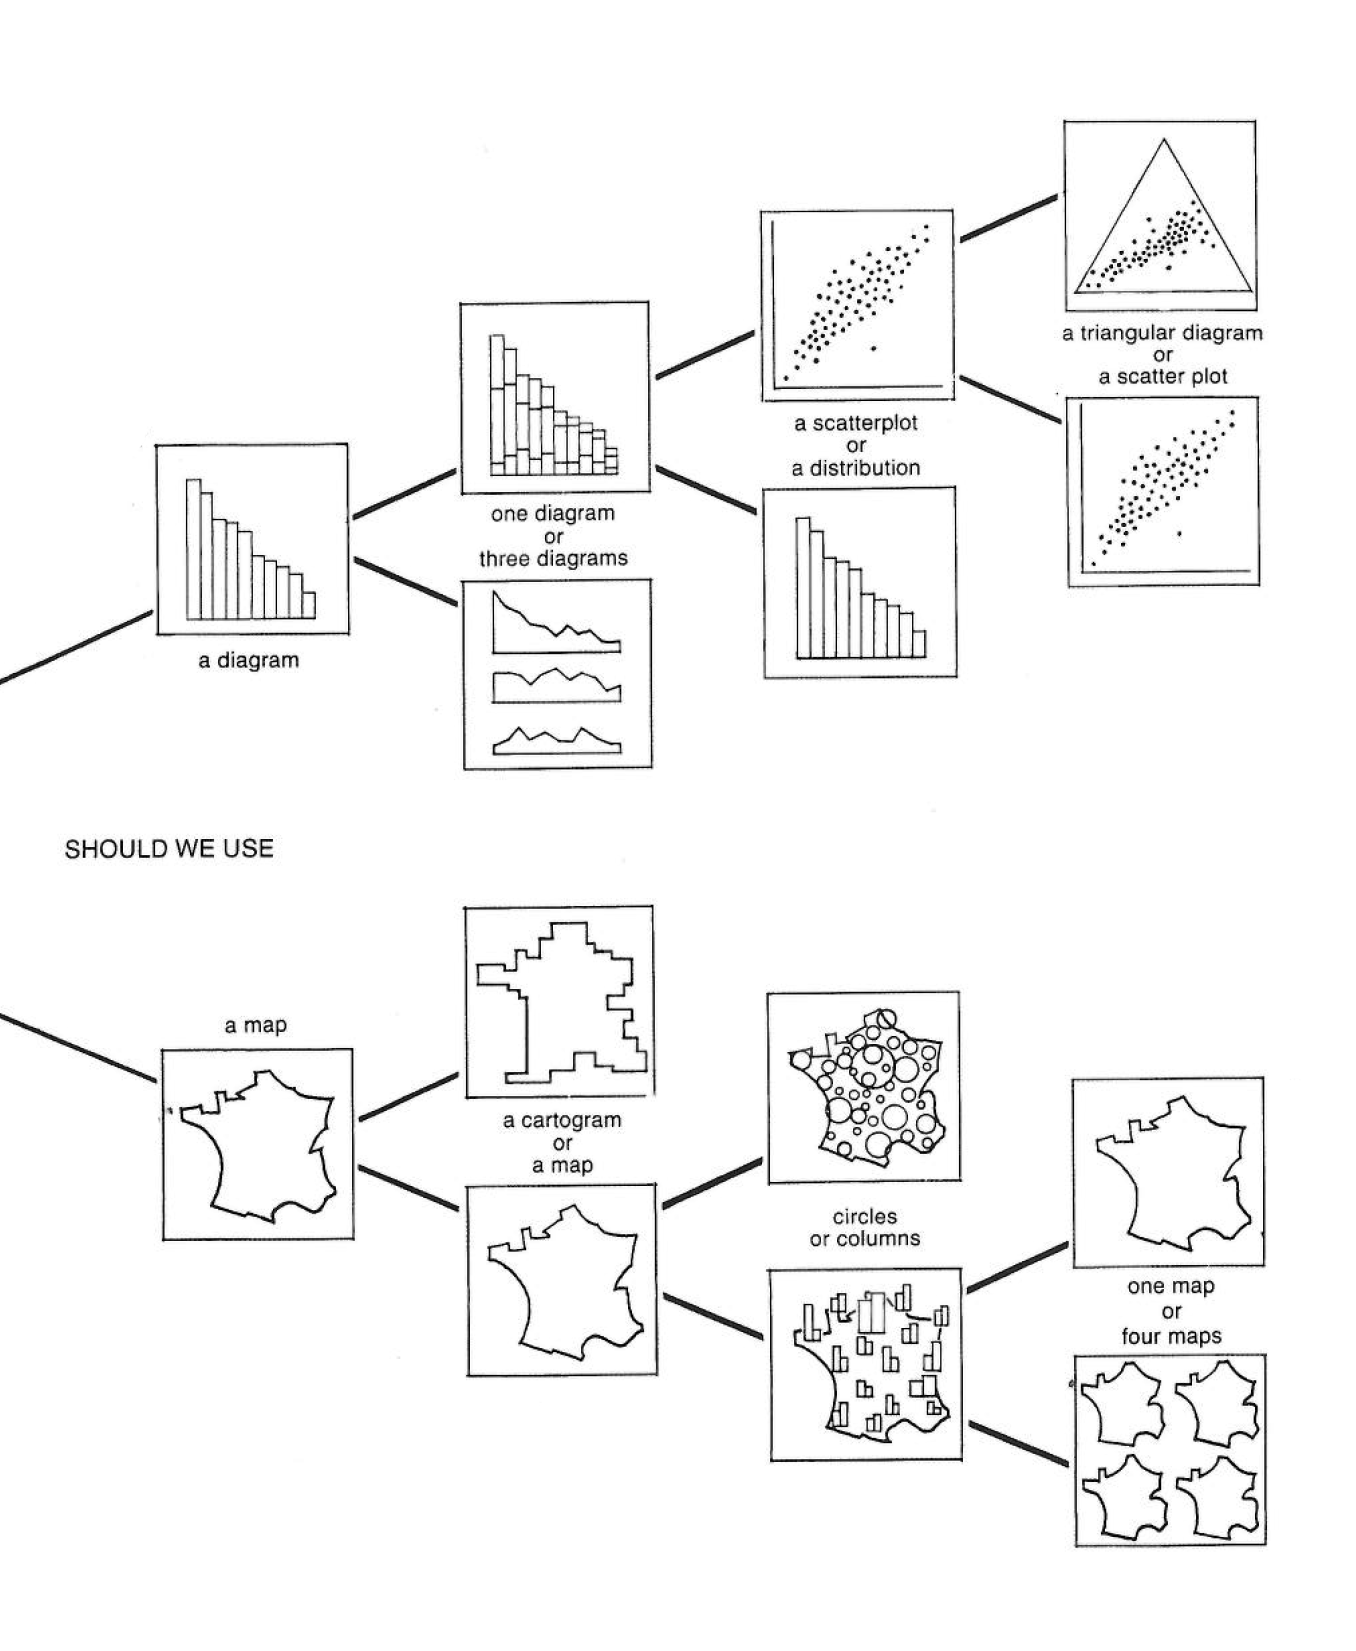
\includegraphics{chart_chooser}
  \caption{From Bertin's Semiology of Graphics \cite{bertin}, this diagram
    illustrates how there are many ways to display the same information about the 1954 Frnech
  workforce.}
  \label{fig:chart_chooser}
\end{figure}

There are almost an overwhelming number of visualizations, and no real correct
choice for any given situation. As figure~\ref{fig:chart_chooser} shows, often
there isn't even a single standout chart for a single dataset; instead the
choice of figure is dependent on the relationships the researcher would like to
extract from the dataset. Is it important to know how many people are in each
department? A bar chart is suited for this, but this data has that information
segmented into sectors - should it be combined or stay separated? Is the
spatial distribution of the workforce something that should be preserved? If
so, how should the sector information be retained? Sectors and space can both
conditional attributes of the data, yielding information on how the workforce
varies when disaggregated into these smaller blocks.

Quite often, it is this disaggregation that is interesting to researchers
because it points to multiple factors that can contribute to the measured
outcome. The difficulty is in figuring out how to visualize this
disaggregation, especially as the data structure grows more complex. Cross
tabulation tables work for a small number of categorical variables, but are
pushed to the limits at n=3 or 4. And most data is not solely categorical,
instead often having quantitative densities of one sort or another. A complex but
important form of quantitative densities are functional densities, where they are drawn from a continuous sample of observations \cite{ramsey2006, ramsey2002, muller2006}. That continuous sample is often over space or time or another parameter or combination thereof, and often it is
important to preserve those functional dependencies in the visualization. For
example, for storm modeling it is important to show the expected time and
location of the rainfall. This survey presents a sampling of visualization
techniques that attempt to illustrate these conditional and functional
relationships within a dataset. 



\begin{table}

\begin{tabular}
                & Distribution           & Density 
   Distribution & P(X|Y),P(A,B,C|E,F,G)  & 
   Density      &              & p(X|Y), p(A,B,C|E,F,G)
\end{tabular}

\caption{The rows represent the known distributions & densities while the
  columns are the distributions and densities that the visualization aims to derive.}
\end{table}

While this survey focuses on data structured in a linear, tabular, or
data cube way\cite{munzner data structure}, it could potentially be expanded to network data where the xi
parameters represent edges in the graph. 


\subfile{sections/distdist.tex}
\subfile{sections/distdens.tex}
\subfile{sections/densdist.tex}
\subfile{sections/densdens.tex}

\section{Conclusion}
\label{sec:conclusion}
When trying to choose a visualization technique for a problem, it is often
crucial to interrogate the questions being asked of the data. What
relationships are important to preserve and which can be discarded? While there
are a what feels like infinite number of visualization techniques, this
visualization task can be rather complicated, especially as the number of
variables or dependencies increases. Interactive tools can help, but most are limited to showing pairwise or a small number of connected interactions. Machine learning can somewhat be used
to explore which variables and dimensions, and therefore which relationships, are worth
exploring further, but often the results of those algorithms need to
be translated to the visual space and those visualizations need to be
understandable. 


\printbibliography
\end{document}
